\documentclass[12pt,a4paper,openright,twoside]{book}
\usepackage[utf8]{inputenc}
\usepackage{disi-thesis}
\usepackage{code-lstlistings}
\usepackage{notes}
\usepackage{shortcuts}
\usepackage{acronym}

\school{\unibo}
\programme{Corso di Laurea
%[Magistrale?]
in Ingegneria e Scienze Informatiche}
\title{
%Fancy Title
Navigazione e Guida Autonoma di Veicoli Aerospaziali: Filtro di Kalman e sue varianti
}
\author{
%Candidate Name
Marco Buda
}
\date{\today}
\subject{
%Supervisor's course name
Metodi Numerici
}
\supervisor{Prof.ssa
%Supervisor Here
Damiana Lazzaro
}
%\cosupervisor{Dott. CoSupervisor 1}
%\morecosupervisor{Dott. CoSupervisor 2}
\session{
%I
II % TODO: verificare
}
\academicyear{
%2022-2023
2024-2025
}

% Definition of acronyms
\acrodef{IoT}{Internet of Thing}
\acrodef{vm}[VM]{Virtual Machine}


\mainlinespacing{1.241} % line spacing in mainmatter, comment to default (1)

\begin{document}

\frontmatter\frontispiece

\begin{abstract}	
Max 2000 characters, strict.
\end{abstract}

\begin{dedication} % this is optional
Optional. Max a few lines.
\end{dedication}

%----------------------------------------------------------------------------------------
\tableofcontents   
\listoffigures     % (optional) comment if empty
\lstlistoflistings % (optional) comment if empty
%----------------------------------------------------------------------------------------

\mainmatter

%----------------------------------------------------------------------------------------
\chapter{Introduction}
\label{chap:introduction}
%----------------------------------------------------------------------------------------

Write your intro here.
\sidenote{Add sidenotes in this way. They are named after the author of the thesis}

You can use acronyms that your defined previously,
such as \ac{IoT}.
%
If you use acronyms twice,
they will be written in full only once
(indeed, you can mention the \ac{IoT} now without it being fully explained).
%
In some cases, you may need a plural form of the acronym.
%
For instance,
that you are discussing \acp{vm},
you may need both \ac{vm} and \acp{vm}.

\paragraph{Structure of the Thesis}

\note{At the end, describe the structure of the paper}

\chapter{State of the art}

\section{I sistemi dinamici} \label{dynsys}

Un sistema dinamico è un qualunque sistema in cui sia individuabile uno stato che evolve come funzione del tempo: $x=f(t)$. \\
Per gli scopi di questa tesi, lo stato verrà rappresentato come un vettore $x\in\mathbb{R}^n$, che raccoglie le variabili di stato (es.: posizione, velocità...), e il tempo verrà considerato come una quantità continua $t\in\mathbb{R}$, eventualmente campionata in determinati istanti $t_k$.

Modellare la realtà a livello macroscopico comporta spesso che $f$ sia non deterministica, per via di fenomeni microscopici. Questo introduce la necessità di effettuare misurazioni periodiche (\textit{measurement}, $z\in\mathbb{R}^m$) per monitorare la reale evoluzione dello stato in presenza di disturbi (\textit{process noise}, $w\in\mathbb{R}^n$). \\
Sfortunatamente, le misurazioni stesse sono soggette ad ulteriori disturbi (\textit{measurement noise}, $v\in\mathbb{R}^m$). \\
Nasce, quindi, l'esigenza di algoritmi che raccolgano ed interpretino i dati misurati per determinare una stima (\textit{state estimate}, $\hat{x}$) dello stato reale (\textit{ground truth}, $x$). Questi algoritmi sono detti, appunto, stimatori.

\section{Il filtro di Kalman}

Il filtro di Kalman~\cite{10.1115/1.3662552} è uno stimatore lineare ricorsivo che minimizza l'errore quadratico medio. \\
L'aspetto ricorsivo si rifà al fatto che ogni stima $\hat{x}_k$ è determinata in base alla stima precedente $\hat{x}_{k-1}$, senza richiedere l'utilizzo esplicito di $\hat{x}_0,\hat{x}_1,...,\hat{x}_{k-2}$. Si tratta di uno dei principali vantaggi del filtro, in quanto riduce sia la complessità temporale che quella spaziale, senza compromettere l'ottimalità. \\
Come anticipato, l'ottimalità è definita dal fatto che l'algoritmo produce la stima $\hat{x}_k$ che minimizza la quantità $\mathbb{E}[\lVert\hat{x}_k-\mathbb{E}[\hat{x}_k]\rVert^2]$ ad ogni passo $k$. \\

Il filtro di Kalman può essere applicato a sistemi dinamici che siano rappresentabili con un modello ricorsivo lineare:
$$x_k=A_kx_{k-1}+B_ku_{k-1}+w_{k-1}$$
dove $A_k$ è la matrice di evoluzione dello stato dal passo $k-1$ al passo $k$ in assenza di disturbi e ``azioni di controllo'', $B_k$ è la matrice che di contributo delle ``azioni di controllo'' (\textit{control input}) $u_{k-1}$ che agiscono dal passo $k-1$ al passo $k$ e $w_{k-1}$ è il \textit{process noise} citato nella sezione \ref{dynsys} che agisce dal passo $k-1$ al passo $k$.

\subsection{Costruzione del filtro}

Si supponga di avere a disposizione 
Nelle formulazioni classiche del filtro di Kalman vengo assunte le seguenti ipotesi

I suggest referencing stuff as follows: \cref{fig:random-image} or \Cref{fig:random-image}

\begin{figure}
    \centering
    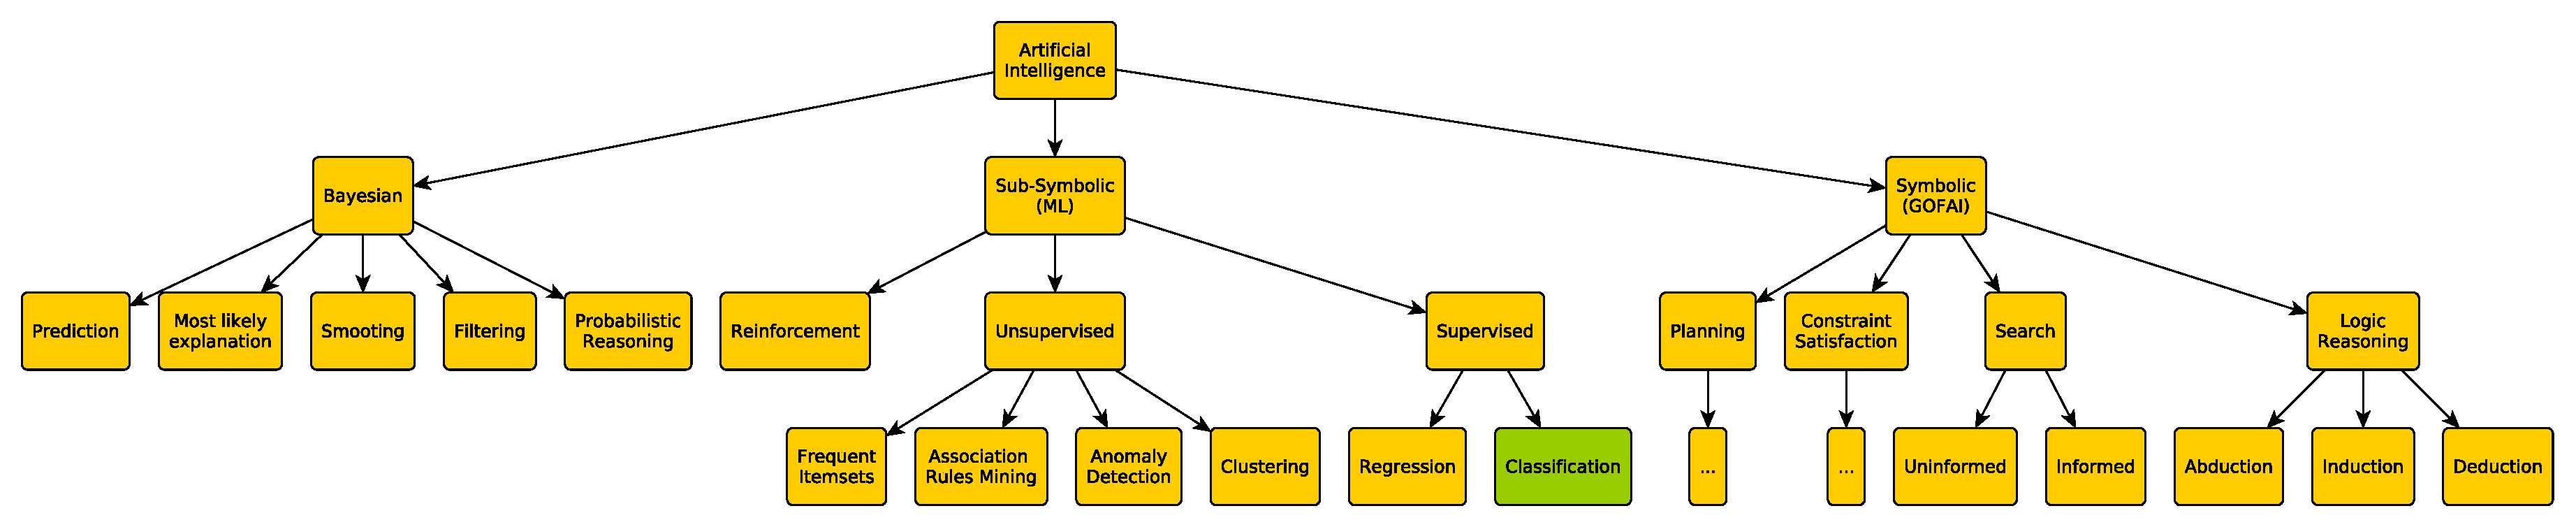
\includegraphics[width=.8\linewidth]{figures/random-image.pdf}
    \caption{Some random image}
    \label{fig:random-image}
\end{figure}

\section{Some cool topic}

\chapter{Contribution}

You may also put some code snippet (which is NOT float by default), eg: \cref{lst:random-code}.

\lstinputlisting[float,language=Java,label={lst:random-code}]{listings/HelloWorld.java}

\section{Fancy formulas here}

%----------------------------------------------------------------------------------------
% BIBLIOGRAPHY
%----------------------------------------------------------------------------------------

\backmatter

% \nocite{*} % Remove this as soon as you have the first citation

\bibliographystyle{alpha}
\bibliography{bibliography}

\begin{acknowledgements} % this is optional
Optional. Max 1 page.
\end{acknowledgements}

\end{document}
